\begin{frame}[fragile]{PVS-Type Definitions}
\begin{lstlisting}
type ConstraintRelationships = PVSType<bool, set of 1..nScs> = 
  params { 
    array[int, 1..2] of 1..nScs: crEdges; % adjacency matrix
    bool: useSPD;
  } in 
  instantiates with "../mbr_types/cr_type.mzn" {
    times -> link_invert_booleans;
    is_worse -> is_worse_cr;
    top -> {};
  };
\end{lstlisting}
\begin{itemize}
\item \texttt{PVSType<S,E>} distinguishes
\begin{itemize}
\item[] Specification type $S$ 
\item[] Element type $E$
\end{itemize} 
\item Combination operation: $\mathtt{times} : S^n \to E$
\item Ordering relation: $\mathtt{isWorse} \subseteq E \times E$
\end{itemize}
\end{frame}

\begin{frame}[fragile]{PVS-Types}
\begin{lstlisting}
type WeightedCsp = PVSType<bool, int> = 
  params {
    int: k; 
    array[1..nScs] of 1..k: weights :: default('1');
  } in  
  instantiates with "../mbr_types/weighted_type.mzn" {
    times -> weighted_sum;
    is_worse -> is_worse_weighted;
    top -> 0;
  };
  
type CostFunctionNetwork = PVSType<0..k> = 
  params {
    int: k :: default('1000'); 
  } in  instantiates with "../mbr_types/cfn_type.mzn" {
    times -> sum;
    is_worse -> is_worse_weighted; 
    top -> 0;
 };
\end{lstlisting}
\end{frame}

\begin{frame}[fragile]{PVS-Instantiation for Weighted-CSp}
\begin{lstlisting}
PVS: cr1 = new WeightedCsp("cr1") {
   soft-constraint c1: 'x + 1 = y' :: weights('2');
   soft-constraint c2: 'z = y + 2' :: weights('1');
   soft-constraint c3: 'x + y <= 3' :: weights('1');
   
   k : '20';
}; 
\end{lstlisting}
\begin{itemize}
\item Weights can be annotated 
\item Or passed as array (\texttt{[2,1,1]}) %\item Aber können wir sie nicht auch berechnen? Aus Constraint Relationships? \pause 
\end{itemize}
\end{frame}


\begin{frame}{Passing between PVS types}\small

\begin{itemize}
\item There are good reasons for \emph{translating} between PVS types
%
\begin{itemize}
\item[-] Ordering should be totalized (e.g. otherwise hard to understand)
\item[-] Data type $xy$ (e.g. sets) not supported by solver/algorithm (think LP/MIP)
\item[-] $\rightarrow$ user is \alert{not} interested in a particular preference data structure but just cares about the solution ordering
%\item[-] Beispiel: Gewichte aus Constraint Relationships für CPLEX
\end{itemize}
% 
\pause 
\vspace*{2ex}
\item Hence, we need \emph{structure-preserving} mappings \pause
\item PVS homomorphism $\varphi : \mathsf{PVS}_{\mathrm{cr}} \to  \mathsf{PVS}_{\mathrm{weighted}}$ \pause 
\item $\mathsf{PVS}_{\mathrm{cr}} = \mathit{PVS}\langle P \rangle = \langle \mathcal{M}^{\mathrm{fin}} (P), \mcup, \supseteq_{\mathsf{SPD}}, \lbag \rbag \rangle$
\begin{itemize}
\item[-] $\varphi(\top_{\mathrm{cr}}) = \top_{\mathrm{weighted}}$ \pause 
\item[-] $\varphi(m \cdot_{\mathrm{cr}} n) = \varphi(m) \cdot_{\mathrm{weighted}} \varphi(n)$ \pause 
\item[-] $m \leq_{\mathrm{cr}} n \rightarrow \varphi(m) \leq_{\mathrm{weighted}} \varphi(n)$ \pause 
\end{itemize}

\end{itemize}
%\begin{center}
%\begin{tikzpicture}
%  \matrix (m) [matrix of math nodes,row sep=3em,column sep=4em,minimum width=2em,ampersand replacement=\&]
%  {
%     \mathit{PVS}\langle P \rangle  \&  \mathit{Weighted}(P) \&  \\
%  };
%      
%  \path[-stealth]
%    (m-1-1) edge node [above] {$\SPDw{}$} (m-1-2)
%;
%
%\end{tikzpicture}
%\end{center}
\begin{textblock*}{3cm}[1,1](\textwidth+.5cm,\textheight-1.3cm)
%\textblockcolour{issegrey!20}
\begin{center}
\begin{tikzpicture}[auto,
                    ->,>=stealth',shorten >=1pt,thick,
                    node distance=.7cm,inner sep=2pt,
                    constraint/.style={circle,fill=black!15,draw,font=\sffamily\small}]
\node[overlay,rectangle callout,callout absolute pointer = {(-3,0.8)},
     draw=isseorange!50,fill=white] at (0,.5) {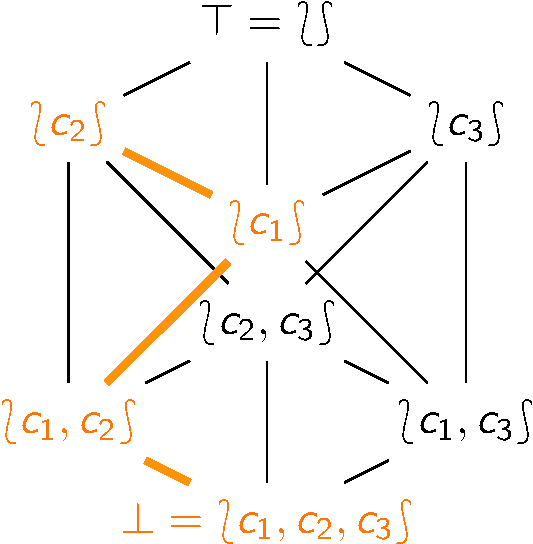
\includegraphics[width=2cm]{img/search-space.pdf}};  
\end{tikzpicture}

\end{center}
\end{textblock*}
\end{frame}

\begin{frame}{Example: Weights for Constraint Relationships}
\begin{figure}
\centering
\begin{tikzpicture}[->,>=stealth',shorten >=1pt,auto,node distance=1.45cm,inner sep=1.5pt,outer sep = 0.0pt, thick] 

\tikzstyle{every node}=[font=\small]

\begin{scope}[xshift=-12cm,yshift=0.0cm]
\node[constraint node, xshift=0.6cm, label=west:{\small 4/13}] (1) {$\mathrm{c_7}$};
\node[constraint node, xshift=1cm, label=east:{\small 2/3}] (3)  [below right of=1] {$\mathrm{c_1}$};
\node[constraint node, label=0:{\small 1/1}] (4) [below left of=3] {$\mathrm{c_2}$};
\node[constraint node, label=0:{\small 1/1}] (8) [below right of=3] {$\mathrm{c_3}$};
\node[constraint node, label=0:{\small 3/4}] (5) [below left of=1, xshift=-.5cm] {$\mathrm{c_4}$};
\node[constraint node, node distance=0.85cm, label=0:{\small 2/2}] (6) [below of=5] {$\mathrm{c_5}$};  
\node[constraint node, node distance=0.85cm,label=0:{\small 1/1}] (7) [below of=6] {$\mathrm{c_6}$};  

\path[every node/.style={font=\sffamily\tiny}]
  (3) edge node [right] {} (1)
  (5) edge node [right] {} (1)
  (4) edge node [right] {} (3)
  (8) edge node [right] {} (3) 	
  (6) edge node [right] {} (5)
  (7) edge node [right] {} (6)    
  ;
        
%\draw [rounded corners, black!45,dashed] (-2.0,-0.5) rectangle (0.3,-3.8);
%\node[yshift=-.75cm] (ag1) at (7){ Agent 1};
    
%\draw [rounded corners, black!45,dashed] (0.6,-0.5) rectangle (4.5,-3.8);
%\node[yshift=-2.45cm] (ag2) at (3) { Agent 2};
\end{scope}

\end{tikzpicture}
\caption{Beispiel mit errechneten Gewichten}
\label{fig:combRelGraph}
\end{figure}


%%% Local Variables:
%%% mode: LaTeX
%%% mode: TeX-PDF
%%% mode: TeX-source-correlate
%%% TeX-master: "../quality-quantity-soft-constraints.tex"
%%% End:


\bgroup\abovedisplayskip=-16pt\belowdisplayskip=4pt
\begin{align*}
  \SPDw{}(c) &\textstyle= 1 + \max_{c' \rightarrow^+ c} \SPDw{}(c') 
\\
  \TPDw{}(c) &\textstyle= 1 + \sum_{c' \rightarrow^+ c} \TPDw{}(c')  
\end{align*}
\egroup

\vspace*{1ex} \small \pause 
\begin{itemize}
\item For ordering $P$ over constraints: PVS $\mathrm{Weighted}(P) = \langle \mathbb{N}, +, \geq, 0 \rangle$
\item $\mathsf{PVS}_{\mathrm{cr}} = \mathit{PVS}\langle P \rangle = \langle \mathcal{M}^{\mathrm{fin}} (P), \mcup, \supseteq_{\mathsf{SPD}}, \lbag \rbag \rangle$
\item $\varphi(\lbag \rbag) = 0$, $\varphi(\lbag c\rbag \mcup C) = \SPDw{}(c) + \varphi(C)$
\end{itemize}



\hfill \cite{Schiendorfer13}
\begin{textblock*}{3cm}[1,1](\textwidth+1cm,\textheight-2.7cm)
%\textblockcolour{issegrey!20}
\begin{center}
\begin{tikzpicture}[auto,
                    ->,>=stealth',shorten >=1pt,thick,
                    node distance=.7cm,inner sep=5pt, 
                    constraint/.style={circle,fill=black!15,draw,font=\sffamily\small}]
\node[overlay,rectangle callout,callout absolute pointer = {(-2,-1)},
     draw=isseorange!50,fill=white] at (0,0) {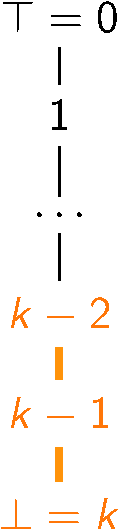
\includegraphics[width=.6cm]{img/search-space-weighted.pdf}};  
\end{tikzpicture}
\end{center}
\end{textblock*}
\end{frame}
%
%\begin{frame}{PVS und Morphismen} \small
%Etwas systematischer \ldots 
%\begin{itemize}
%\item $\mathsf{PVS}_{\mathrm{cr}} = \mathit{PVS}\langle P \rangle = \langle \mathcal{M}^{\mathrm{fin}} (P), \mcup, \supseteq_{\mathsf{SPD}}, \lbag \rbag \rangle$
%\item PVS-Homomorphismus $\varphi : \mathsf{PVS}_{\mathrm{cr}} \to  \mathsf{PVS}_{\mathrm{weighted}}$ \pause 
%\begin{itemize}
%\item[-] $\varphi(\top_{\mathrm{cr}}) = \top_{\mathrm{weighted}}$ \pause 
%\item[-] $\varphi(m \cdot_{\mathrm{cr}} n) = \varphi(m) \cdot_{\mathrm{weighted}} \varphi(n)$ \pause 
%\item[-] $m \leq_{\mathrm{cr}} n \rightarrow \varphi(m) \leq_{\mathrm{weighted}} \varphi(n)$ \pause 
%\end{itemize}
%
%\vspace*{2ex}
%
%\item Beispiel: $\varphi(\lbag \rbag) = 0$, $\varphi(\lbag c\rbag \mcup C) = \SPDw{}(c) + \varphi(C)$
%
%\vspace*{2ex}
%
%\pause 
%\item Warum überhaupt Morphismen?
%\begin{itemize}
%\item[-] Ordnung soll bewusst totalisiert werden
%\item[-] Datentyp $xy$ (z.B. Mengen) wird von Solver/Algorithmus nicht unterstützt
%\item[-] $\rightarrow$ Benutzer interessiert \alert{nicht} konkrete Datenstruktur sondern nur die Erhaltung der gewünschten Ordnung
%\end{itemize}
%\end{itemize}
%%\begin{center}
%%\begin{tikzpicture}
%%  \matrix (m) [matrix of math nodes,row sep=3em,column sep=4em,minimum width=2em,ampersand replacement=\&]
%%  {
%%     \mathit{PVS}\langle P \rangle  \&  \mathit{Weighted}(P) \&  \\
%%  };
%%      
%%  \path[-stealth]
%%    (m-1-1) edge node [above] {$\SPDw{}$} (m-1-2)
%%;
%%
%%\end{tikzpicture}
%%\end{center}
%\begin{textblock*}{3cm}[1,1](\textwidth+.5cm,\textheight-5.3cm)
%%\textblockcolour{issegrey!20}
%\begin{center}
%\begin{tikzpicture}[auto,
%                    ->,>=stealth',shorten >=1pt,thick,
%                    node distance=.7cm,inner sep=2pt,
%                    constraint/.style={circle,fill=black!15,draw,font=\sffamily\small}]
%\node[overlay,rectangle callout,callout absolute pointer = {(-3,0.8)},
%     draw=isseorange!50,fill=white] at (0,.5) {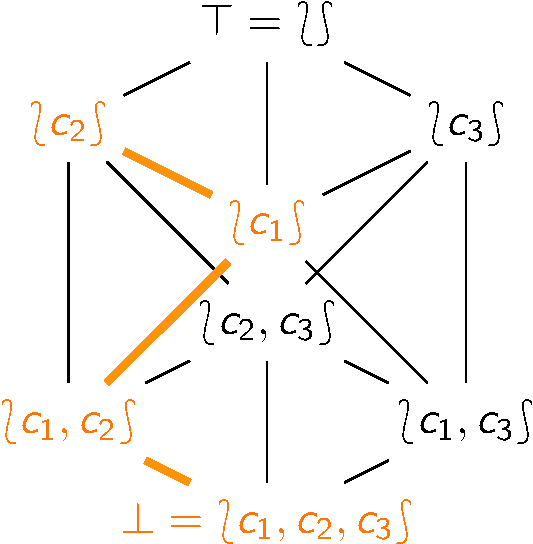
\includegraphics[width=2cm]{img/search-space.pdf}};  
%\end{tikzpicture}
%
%\end{center}
%\end{textblock*}
%\end{frame}


\begin{frame}{Looking for freedom \ldots} \small

\begin{center}
\begin{tikzpicture}[auto,->,
                    >=stealth',shorten >=1pt,thick,
                    node distance=.7cm,inner sep=2pt,
                    constraint/.style={circle,fill=black!15,draw,font=\sffamily\small},
                    bg/.style={shape=rectangle, rounded corners,
    draw, align=center,
    top color=white, bottom color=issegrey!15},
                    pvs/.style={shape=rectangle, rounded corners,
    draw=isseorange!50,fill=white, align=center}]
\node [anchor=west] at (0, .5) {$\mathrm{Cat}: \mathrm{POSet}$};
\node [anchor=west] at (0, -.5) {$\mathrm{Cat}: \mathrm{PVS}$};

\draw [dashed,-] (0,0) -- (11,0);

 \node[bg,text width=2.7cm, text height=1.5cm] at (5,1.6) {};
 \node[anchor=west] at (3.6,2.1) {$P$};
 
\node[constraint node] (1) at (5, 2)                   {$\mathrm{c}_1$};
\node[constraint node] (2) at ($ (1) + (-0.8, -0.8) $) {$\mathrm{c}_2$};  
\node[constraint node] (3) at ($ (1) + ( 0.8, -0.8) $) {$\mathrm{c}_3$};  
%  
\path[every node/.style={font=\sffamily\tiny}]
  (2) edge (1)
  (3) edge (1)
  ;
 
\onslide<2-> { 
\node[pvs,text width=3.5cm,anchor=north west, text height=2.8cm] at (0.5,-1) {};
 \node[anchor=west] at (0.5,-1.3) {$\mathit{Weighted}(P)$};
  \node[anchor=west] at (0.5,-3.6) {$\langle \mathbb{N}, +, \geq, 0 \rangle$};
  
\node[constraint node,label=west:2] (w1) at (2, -2)                   {$\mathrm{c}_1$};
\node[constraint node,label=west:1] (w2) at ($ (w1) + (-0.8, -0.8) $) {$\mathrm{c}_2$};  
\node[constraint node,label=west:1] (w3) at ($ (w1) + ( 0.8, -0.8) $) {$\mathrm{c}_3$};  
\node at (3.5, -2.3) {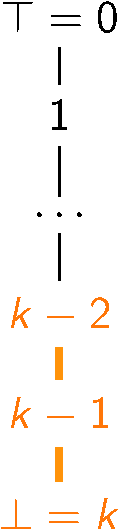
\includegraphics[width=.45cm]{img/search-space-weighted.pdf} }; 

%  
\path[every node/.style={font=\sffamily\tiny}]
  (w2) edge (w1)
  (w3) edge (w1)
  ;
}

\onslide<2->{
\draw [CornflowerBlue] (5,0.7) -- (2,-1);
\node [CornflowerBlue] at (4.2,-0.5) {$\mu(c) = \SPDw{}(c)$};
}  
 
\onslide<3->{
\node[pvs,text width=4.5cm,anchor=north west, text height=2.8cm] at (5.7,-1) {};
\node[anchor=west] at (5.7,-1.3) {$\mathit{PVS}\langle P \rangle $};
\node[anchor=west] at (5.7,-3.6) {$\langle \mathcal{M}^{\mathrm{fin}} (P), \mcup, \supseteq_{\mathsf{SPD}}, \lbag \rbag \rangle$};

\node[constraint node,label=west:$\lbag \mathrm{c}_1 \rbag$] (p1) at (7, -2)                   {$\mathrm{c}_1$};
\node[constraint node,label=east:$\lbag \mathrm{c}_2 \rbag$] (p2) at ($ (p1) + (-0.8, -0.8) $) {$\mathrm{c}_2$};  
\node[constraint node,label=north:$\lbag \mathrm{c}_3 \rbag$] (p3) at ($ (p1) + ( 0.8, -0.8) $) {$\mathrm{c}_3$};  
\node at (9.2, -2.3) {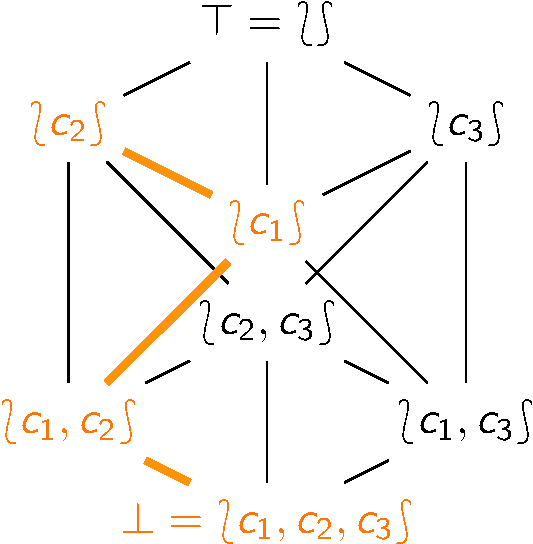
\includegraphics[width=2cm]{img/search-space.pdf} }; 
%  
\path[every node/.style={font=\sffamily\tiny}]
  (p2) edge (p1)
  (p3) edge (p1)
  ;
}
 
\onslide<3->{ 

\draw [isseorange] (5,0.7) -- (8,-1);
\node [isseorange] at (8.7,-0.5) {$\eta(c) = \lbag c \rbag$};
}

%\onslide<6->{
%\draw [issegrey] (5.7,-2) to [bend right] (4.2,-2);  
%\node [issegrey] at (5,-1.5) {$(\SPDw{})^\#$};
%}

%\onslide<7->{
%\draw [issegrey]  (4.2,-2.5) to [bend right] (5.7,-2.5);   
%\node [issegrey] at (5,-3) {?};
%}
\end{tikzpicture}
\end{center}

\end{frame}


\begin{frame}[fragile]{Morphisms in MiniBrass}
\begin{lstlisting}
% import from a library 
morph ConstraintRelationships -> WeightedCsp: ToWeighted = 
  params {
    k = 'mbr.nScs * max(i in 1..mbr.nScs) (mbr.weights[i]) ';
    weights = calculate_cr_weights;
  } in id; % "in" denotes the function applied to each soft constraint 
\end{lstlisting}
\begin{lstlisting}   
PVS: cr1 = new ConstraintRelationships("cr1") {
   soft-constraint c1: 'x + 1 = y';
   soft-constraint c2: 'z = y + 2';
   soft-constraint c3: 'x + y <= 3';
   
   crEdges : '[| mbr.c2, mbr.c1 | mbr.c3, mbr.c1 |]';
   useSPD: 'false' ;
}; 
solve ToWeighted(cr1);
\end{lstlisting}
\begin{Verbatim}[fontsize=\small]
Solution: x = 1; y = 2; z = 1
Valuations: overall = 1
\end{Verbatim}
\begin{textblock*}{3cm}[1,1](\textwidth+0.5cm,\textheight+0.3cm)
%\textblockcolour{issegrey!20}
\begin{center}
\begin{tikzpicture}[auto,
                    ->,>=stealth',shorten >=1pt,thick,
                    node distance=.7cm,inner sep=2pt,
                    constraint/.style={circle,fill=black!15,draw,font=\sffamily\small}]
\node[constraint node,label=west:2] (1) at (0, 0)                   {$\mathrm{c}_1$};
\node[constraint node,label=west:1] (2) at ($ (1) + (-0.8, -0.8) $) {$\mathrm{c}_2$};  
\node[constraint node,label=west:1] (3) at ($ (1) + ( 0.8, -0.8) $) {$\mathrm{c}_3$};  
%  
\path[every node/.style={font=\sffamily\tiny}]
  (2) edge (1)
  (3) edge (1)
  ;
  

\end{tikzpicture}
\begin{Verbatim}[fontsize=\small]
c1: 'x + 1 = y';
c2: 'z = y + 2';
c3: 'x + y <= 3';   
\end{Verbatim}

\end{center}
\end{textblock*}

\end{frame}

\begin{frame}[fragile]{PVS Combinations: Pareto} \small
With PVSs $M$ and $N$ we can build the \emph{direct product} $M \times N$ 
\[
(m, n) \leq_{M \times N} (m', n') \leftrightarrow m \leq_M m' \wedge n \leq_N n'
\]
bilden. Entspricht der \emph{Pareto}-Ordnung
\begin{lstlisting}
% in MZN-file: var 1..10: x; var 1..10: y;
PVS: cfn1 = new CostFunctionNetwork("cfn1") {
   soft-constraint c1: 'y' ;
   k : '20';
}; 

PVS: cfn2 = new CostFunctionNetwork("cfn2") {
   soft-constraint c1: 'x' ;
   k : '20';
}; 

solve cfn1 pareto cfn2; % returns x = 1, y = 1
\end{lstlisting}
\end{frame}

\begin{frame}[fragile]{PVS Combinationen: Lex}
Additionally, we have the \alert{lexicographic} product $M \ltimes N$ 
\[
(m, n) \leq_{M \ltimes N} (m', n') \leftrightarrow (m <_M m') \vee (m = m' \wedge n \leq_N n')
\]
Allows for strict hierarchies
\begin{lstlisting}
% in MZN-file: var 1..3: x; var 1..3: y;
PVS: cfn1 = new CostFunctionNetwork("cfn1") {
   soft-constraint c1: 'x' ;
   soft-constraint c2: '3 - y' ;
   k : '20';
}; 
PVS: cfn2 = new CostFunctionNetwork("cfn2") {
   soft-constraint c1: 'y' ;
   soft-constraint c2: '3 - x' ;
   k : '20';
};
solve cfn1 lex cfn2; % returns x = 1, y = 3
% dually cfn2 lex cfn1 yields x = 3, y = 1 
\end{lstlisting}
\end{frame}

\begin{frame}{Complex Valuation Structures}
\fontsize{8pt}{7.2}\selectfont
\tikzset{
   main node/.style={rectangle,
                     rounded corners,
   					 fill=black!15,
   					 draw,
   					 minimum width=3.5em,
   					 text centered,
                     inner sep=2.5pt,	 
   					 font=\sffamily
   					},
   treestyle/.style={rectangle,fill=black!15,draw,font=\sffamily},
   constraint/.style={circle,fill=black!15,draw,font=\sffamily\small},
   constraint_satisfied/.style = {constraint, fill=white},
   constraint_violated/.style = {constraint, fill=black!25},
}

\begin{figure}[t]
\centering
\begin{tikzpicture}[->,>=stealth',shorten >=1pt,auto,node distance=1.45cm,inner sep=1.5pt,outer sep = 0.0pt, thick] 
%\tikzstyle{every node}=[font=\tiny]
\begin{scope}[xshift=-6.0cm,yshift=-4.0cm]
\node[main node, style={font=\sffamily\footnotesize}] at (0.1,1.5) {\minMaxViolation[1]};
\node[main node, style={font=\sffamily\footnotesize}] at (3.2,1.5) {\minMaxViolation[2]};
\node[main node, style={font=\sffamily\footnotesize}] at (6.3,1.5) {\minMaxViolation[3]};

\draw [rounded corners,dashed,black!45] (-2,2) rectangle (9.0,1);
\node[text width=3cm, anchor=west, right] at (-2.9, 1.5) { \hLevelOrg{1} };
\draw [rounded corners,dashed,black!45] (-2,0.8) rectangle (9.0,-2.65);
\node[text width=4cm, anchor=west, right] at (-2.9, -0.75) { \hLevelOrg{2} };

% bio
\draw [black!85,fill=forestgreen!35] (-1.8,0.6) rectangle (1.8,-2.5);
\node[main node, style={font=\sffamily\footnotesize}] (5) at (0.05,-0.4) {\gasFull};
\node[main node, style={font=\sffamily\footnotesize}] (6) [below left of=5,xshift=5.4] {\ecoSweet};
\node[main node, style={font=\sffamily\footnotesize}] (7) [below right of=5,xshift=-3.1] {\onOff};
%\node[main node, style={font=\sffamily\footnotesize},double] (hardConstraint) [below left of=7,xshift=-3.1,yshift=7] {$\mathsf{maxProd}$};
\node[text width=4cm, anchor=west, left] at (2.3, 0.3) { \textbf{ConstraintRel.:}  $\mathtt{\biogas}$ $(b)$ };
%\node[text width=2cm, anchor=west, left] at (0.4, 0.3) { CR \textsc{TPD} };

% EV
\draw [black!85,fill=black!35] (2.0,0.6) rectangle (5.6,-2.5);
\node[main node, style={font=\sffamily\footnotesize}] (3) at (2.80,-0.4) {\prefBatteryLevel};
\node[main node, style={font=\sffamily\footnotesize}] (4) at (4.58,-0.4)  {\earlyBird};
\node[main node, style={font=\sffamily\footnotesize}] (8) [below right of=3] {\limitBatteryUsage};
\node[text width=3cm, anchor=west, left] at (5.2, 0.3) { \textbf{ConstraintRel.:}  $\mathtt{\ev}$ $(c)$ };
%\node[text width=2cm, anchor=west, left] at (4.3, 0.3) { CR };
%\node[text width=1cm, anchor=east, left] at (5.3, -2.3) { \textsc{SPD} };

% thermal
\draw [black!85,fill=thermicred!25] (5.8,0.6) rectangle (8.8,-2.5);
\draw [rounded corners,dashed,black!45] (5.9,0) rectangle (8.7,-1.3);
\node[text width=4cm, anchor=west, right] at (5.9, 0.2) { \hLevelThermal{1} };
\draw [rounded corners,dashed,black!45] (5.9,-1.8) rectangle (8.7,-2.4);
\node[text width=4cm, anchor=west, right] at (5.9, -1.6) { \hLevelThermal{2} };
\node[main node, style={font=\ttfamily\footnotesize}] (10) at (6.9,-0.4) {\ecoOpt};
\node[main node, node distance=0.85cm, style={font=\sffamily\footnotesize}] (11) at (6.98,-1.0) {\inertia};
\node[main node, node distance=0.85cm, style={font=\sffamily\footnotesize}] (12) at (6.98,-2.1) {\ecoGood};
\node[text width=4cm, anchor=west, right] at (7.1, 0.3) { $\mathtt{\thermal}$ $(d)$ };

\node[text width=2cm, anchor=west, left] at (10, -0.7) { \textbf{CFN:} \\ $\mathtt{h1}$ };

\node[text width=2cm, anchor=west, left] at (10.1, -2.1) { \textbf{CFN:} \\ $\mathtt{h2}$ };

\node[text width=2cm, anchor=west, left] at (10.1, 1.4) { \textbf{CFN:} \\ $\mathtt{orga}$ };

\path[every node/.style={font=\sffamily\tiny}]
  (8) edge node [right] {} (3)
  (8) edge node [right] {} (4)
  (6) edge node [right] {} (5)
  (7) edge node [right] {} (5)
;
\end{scope}

% \begin{scope}[xshift=-0.2cm,yshift=-0.9cm]
% \node[text width=9cm,left] at (0.0, 0.0) {%
% \begin{itemize}[itemsep=2pt]
%   \item something interesting
% \end{itemize}
% };
% \end{scope}

\end{tikzpicture}
%\caption{Case study depicting individual and organizational preference specifications in context.}
\label{fig:preferencesCaseStudy}
\end{figure}
  



%%% Local Variables:
%%% mode: LaTeX
%%% mode: TeX-PDF
%%% mode: TeX-source-correlate
%%% TeX-master: "../quality-quantity-soft-constraints.tex"
%%% End:


\onslide<1->{
The valuation structure for this problem:
\vspace*{2ex}

\qquad $
  P_{\mathtt{org}_1} \ltimes (P_{\prosumer{\biogas}} \times P_{\prosumer{\ev}} \times (P_{\prosumer{\thermal}}^1 \ltimes P_{\prosumer{\thermal}}^2))
$
}

\hfill \small \cite{SchiendorferPvs2015}
%
%\begin{textblock*}{7.5cm}[1,1](\textwidth+3.8cm,\textheight-0.13cm)
%\begin{itemize}
%%\item[] \textsc{SPD} \ldots Single-Pred.-Dom.
%%\item[] \textsc{TPD} \ldots Single-Pred.-Dom.
%\item[] \textsc{SUM} \ldots Sum of Errors
%\item[] \textsc{WC} \ldots Worst-Case Error
%
%
%\end{itemize}
% \end{textblock*}
\end{frame}